\documentclass{article}

\usepackage{fontspec}                % font for emoji
\newfontfamily\DejaSans{DejaVu Sans}

\usepackage{arxiv}

\usepackage[utf8]{inputenc} % allow utf-8 input
\usepackage[T1]{fontenc}    % use 8-bit T1 fonts
\usepackage{hyperref}       % hyperlinks
\usepackage{url}            % simple URL typesetting
\usepackage{booktabs}       % professional-quality tables
\usepackage{amsfonts}       % blackboard math symbols
\usepackage{nicefrac}       % compact symbols for 1/2, etc.
\usepackage{microtype}      % microtypography
\usepackage{lipsum}		    % Can be removed after putting your text content
\usepackage{graphicx}
\usepackage{natbib}
\usepackage{doi}            % hyperlink to doi.org
\usepackage{enumitem}       % itemize settings
\usepackage{cleveref}       % reference section with capital letter
\usepackage{xcolor}         % additional colors for hypersetup
\usepackage{booktabs}       % beauful tables
\usepackage{caption}        % table caption margin
\usepackage{subcaption}     % images next to each other
\usepackage{placeins}       % floatbarrier
\usepackage[outputdir=build]{minted} % code insertion

\captionsetup[table]{skip=10pt}          % table caption margin
\setlist[itemize]{noitemsep, topsep=0pt} % no space between itemize
\hypersetup{
    colorlinks=true,
    citecolor=violet,
    linkcolor=violet,
    filecolor=violet,      
    urlcolor=black,
}

\title{A hybrid approach for news recommender system using optimization methods}

%\date{September 9, 1985}	% Here you can change the date presented in the paper title
%\date{} 					% Or removing it

\author{
    {
\includegraphics[scale=0.07]{./images/spbu.png}\hspace{1mm}Alexander Smirnov}\\
	Department of Information and Analytical Systems\\
	Saint Petersburg State University\\
	Russia, Saint Petersburg\\
	\texttt{ru.alexander.smirnov@gmail.com} \\
	\And
	{
\includegraphics[scale=0.07]{images/spbu.png}\hspace{1mm}Elena Mikhailova} \\
	Department of Information and Analytical Systems\\
	Saint Petersburg State University\\
	Russia, Saint Petersburg\\
	\texttt{e.mikhaylova@spbu.ru} \\
	%% \AND
	%% Coauthor \\
	%% Affiliation \\
	%% Address \\
	%% \texttt{email} \\
	%% \And
	%% Coauthor \\
	%% Affiliation \\
	%% Address \\
	%% \texttt{email} \\
	%% \And
	%% Coauthor \\
	%% Affiliation \\
	%% Address \\
	%% \texttt{email} \\
}

% Uncomment to remove the date
%\date{}

% Uncomment to override  the `A preprint' in the header
%\renewcommand{\headeright}{Technical Report}
%\renewcommand{\undertitle}{Technical Report}
\renewcommand{\shorttitle}{Recommender System}

\hypersetup{
    pdftitle={A hybrid approach for news recommender system using optimization methods},
    pdfsubject={recommender systems},
    pdfauthor={Alexander Smirnov, Elena Mikhailova},
    pdfkeywords={Recommender Systems, Optimizations},
}

\begin{document}

\maketitle

\begin{abstract}


    Recommender system is an essential part of any social media application. Most recommender systems now use a hybrid approach, combining collaborative filtering, content-based filtering, and other approaches. Most common problems in the field of hybrid recommenders are cold start and data sparsity \citep{overview}. In this paper we address the abovementioned problems by proposing a hybrid weighted news recommender system which combines different approaches.

\end{abstract}


\keywords{hybrid recommender systems \and content-based recommender \and collaborative recommender \and optimizations}



\section{Introduction}

    Recommender system is a crucial part of every application that operates with content and user activity. Enormous amount of information leads to the problem that user is not able to find relevant content.

    Common approaches, such as collaborative filtering, has its own problems: cold start, scalability and data sparsity. Content-based approaches suffer from the fact that we have to somehow represent recommended item in feature space.
    
    To be consistent during the paper we list some domain specific vocabulary with their meanings:

        \begin{itemize}
            \item Rating: expression or preference

                \begin{itemize}
                    \item explicit (direct from user, e.g. user rated film)
                    \item implicit (inferred from user activity, e.g. user stopped watching movie after 5 minutes)
                \end{itemize}
            \item Prediction: estimate of preference
            \item Recommendation: selected items for user
            \item Content: attributes, text, etc; everything about item
        \end{itemize}


    The remainder of this paper is organized as follows:
    
        \begin{itemize}
            \item \Cref{sec:related} describes the relevant related work
            \item \Cref{sec:input} describes input data
            \item \Cref{sec:overview} explains our modular design and architecture
            \item \Cref{sec:implementation} describes the implementation of the algorithms in a real system
            \item \Cref{sec:evaluation} provides tests and experiments validating
our system’s results
            \item \Cref{sec:further} explains future work
            \item \Cref{sec:summary} presents conclusions
        \end{itemize}



\section{Related work}
\label{sec:related}

According to the study \citep{progress}, deep learning techniques are not supposed to beat conceptually and computationally simpler algorithms, so we won't touch them.

Our goal is to choose optimal algorithm for each of the following tasks:

\begin{itemize}
    \item \textbf{Collaborative filtering}: generating predictions about the interests of a user by collecting preferences or taste information from other users. It is based on the assumption that if a person A has the same opinion as a person B on an issue, A is more likely to have B's opinion on a different issue than that of a randomly chosen person
    \item \textbf{Content-based filtering}:
    \item \textbf{Session filtering}:
    \item \textbf{Popularity filtering}:
    \item \textbf{Demographic filtering}:
    \item \textbf{Time-based filtering}:
\end{itemize}

We face the problem that millions of news are theoretically suitable for being recommended, so it is not correct to use abovementioned methods on such large corpus of data. Instead, as stated in \citep{youtube} paper, we want to implement \texttt{candidate generation} $\to$ \texttt{ranking} pipeline to reduce number of candidates.



\subsection{Collaborative filtering}

There were many studies on this topic, but paper \citep{evaluation} proves that well-tuned basic SVD++ approach beats newely presented algorithms.



\section{Input data}
\label{sec:input}

As we solving domain specific task, we have domain specific data.

\subsection*{metadata}

\begin{table}[h]
    \centering
    % \resizebox{\textwidth}{!}{
    \begin{tabular}{ccccc}
        \toprule

        \emph{item\_id} & \emph{date} & \emph{source\_id} & \emph{category}\\\midrule

        1 & 2021-01-08 22:08:39 & 9  & politics, conflicts\\
        2 & 2021-01-09 10:28:58 & 5  & IT, social media\\
        3 & 2021-01-09 14:20:34 & 12 & accident\\
        \vdots & \vdots & \vdots & \vdots \\\bottomrule


     \hline
    \end{tabular}
    % }

    \caption{news metadata}
    \label{tab:meta}
\end{table}


\begin{itemize}
    \item \emph{source\_id}: source of news item
\end{itemize}


\subsection*{content}

\begin{table}[h]
    \centering
    \resizebox{\textwidth}{!}{
    \begin{tabular}{cll}    \toprule

        \emph{item\_id} &  \emph{news title} & \emph{news content} \\\midrule

    1  &  Azerbaijan denies reports on construction of Turkish air bases in the country & Information that Turkey will create air bases ...        \\
    2  &  Durov announced the massive transition of WhatsApp users to Telegram          & Telegram developer Pavel Durov said in his channel ...   \\
    3  &  Passenger plane that disappeared from radar crashed                           & Passenger plane taking off from Jakarta, disappeared ... \\
    \vdots & \vdots & \vdots \\\bottomrule


     \hline
    \end{tabular}
    }

    \caption{news item}
    \label{tab:item}
\end{table}

\subsection*{shows \& views}

\begin{table}[h]
    \parbox{.45\textwidth}{
        \centering
        \begin{tabular}{ccc}
            \toprule

            \emph{user\_id} & \emph{item\_id} \\\midrule
            10 & 1  \\
            10 & 2  \\
            23 & 1  \\
            23 & 3  \\
            23 & 2  \\
            38 & 3  \\
            38 & 1  \\
            \vdots & \vdots  \\\bottomrule
        \end{tabular}
        \caption{news shows}
        \label{tab:show}
    }
    \hfill
    \parbox{.45\textwidth}{
        \centering
        \begin{tabular}{ccc}
            \toprule

            \emph{user\_id} & \emph{item\_id} \\\midrule
            10 & 1  \\
            10 & 2  \\
            23 & 1  \\
            38 & 3  \\
            \vdots & \vdots  \\\bottomrule
        \end{tabular}
        \caption{news views}
        \label{tab:view}
        }
\end{table}   


\begin{itemize}
    \item \emph{shows}: if \emph{item\_id} was shown to the \emph{user\_id}
    \item \emph{views}: if \emph{item\_id} was clicked by the \emph{user\_id}
\end{itemize}



\subsection*{emotions \& comments}

There is an option to react on item via leaving emotion and/or writing a comment.

\begin{table}[h]
    \parbox{.45\textwidth}{
        \centering
        \begin{tabular}{ccc}
            \toprule

            \emph{user\_id} & \emph{item\_id} & \emph{emotion\_id} \\\midrule
            10 & 1 & 1  \\
            10 & 2 & 3        \\
            23 & 1 & 3        \\
            38 & 3 & 2        \\
            \vdots & \vdots & \vdots  \\\bottomrule

        \end{tabular}
        \caption{users' emotions}
        \label{tab:emotion}
    }
    \hfill
    \parbox{.45\textwidth}{
        \centering
        \resizebox{0.45\textwidth}{!}{
        \begin{tabular}{ccc}
            \toprule

            \emph{user\_id} & \emph{item\_id} & \emph{comment} \\\midrule
            10 & 1 & that's great  \\
            10 & 1 & wish it will continue        \\
            23 & 2 & whatsapp is not competetive anymore        \\
            \vdots & \vdots & \vdots  \\\bottomrule

        \end{tabular}
    }
        \caption{users' comments}
        \label{tab:comment}
        }
\end{table}   

\begin{itemize}
    \item \emph{emotion\_id}: one of \{{\DejaSans 😄, 😲, 😞, 😡, ♥ }\}
\end{itemize}


% \FloatBarrier


\subsection*{users' subscriptions}

If \emph{user\_id} subscribed to the \emph{source\_id}.

\begin{table}[h]
    \centering
    \begin{tabular}{cc}
        \toprule

        \emph{user\_id} & \emph{source\_id} \\\midrule

        10 & 9  \\
        23 & 5  \\
        \vdots & \vdots  \\\bottomrule

    \end{tabular}

    \caption{users' subscriptions}
    \label{tab:subscriptions}
\end{table}




\newpage
\section{Overview of our approach}
\label{sec:overview}

Out goal is to combine state-of-the-art approaches in recommender systems.

Solution consists of 2 parts:

\begin{itemize}
    \item \textbf{Candidate generation}: lowering number of items to recommend. These candidates are intended to be generally relevant to the user with high precision. The candidate generation part only provides broad personalization
    \item \textbf{Ranking}: applying state-of-the-art algorithms to rank candidates generated on previous step
\end{itemize}

Architecture provided below on \cref{fig:architecture}:

\begin{figure}[h]
    \centering
    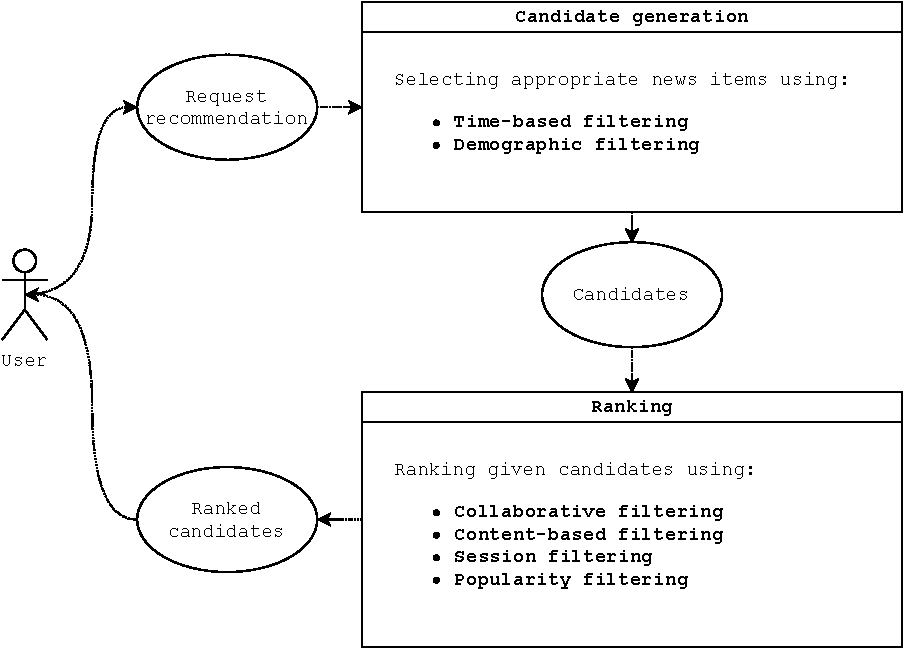
\includegraphics[width=0.8\textwidth]{./images/architechture.pdf}
    \caption{architecture}
    \label{fig:architecture}
\end{figure}

Candidate generation stage not only filters items, but also attaches weight to items.

\subsection{Candidate generation components overview}

Goal of candidate generation step is to remove generally irrelevant items so furher algorithms won't suffer from the amount of data. Both time-based filtering and content-based filtering have their own weight at start. As user more interacting with the system, content-based filtering increasing its weight.

Using recommenders described below, we attach score to each item and pick top $n$ (e.g. $50 000$) items.

\subsubsection{Time-based filtering}

As we operating with news data, first filter is the time filter. This part consists of 2 steps:

\begin{itemize}
    \item \textbf{Filtering}: remove all items which are older than 3 days
    \item \textbf{Ranking}: attach weights to all items left from filtering
\end{itemize}

For ranking we will use following formula:

$$r_i = \frac{(v_i - 1)}{(t - t_i + 2)^G}$$


\begin{itemize}
    \item $r_i$ -- score for $item_i$
    \item $v_i$ -- number of views of $item_i$
    \item $t$ -- time right now, $t_i$ -- time of creation of $item_i$, $t - t_i$ -- hours passed since item created
    \item $G$ -- gravity factor
\end{itemize}

The score decreases as $t - t_i$ increases, meaning that older items will get lower and lower scores. $v_i$ gets substracted by $-1$ to negate submitter's view. $t - t_i$ increased by $2$ so even if $t - t_i = 0$ gravity factor $G$ will take effect.


Below are show dependencies between score and hours since creation:

\begin{figure}[h]
  \begin{subfigure}[b]{0.5\textwidth}
    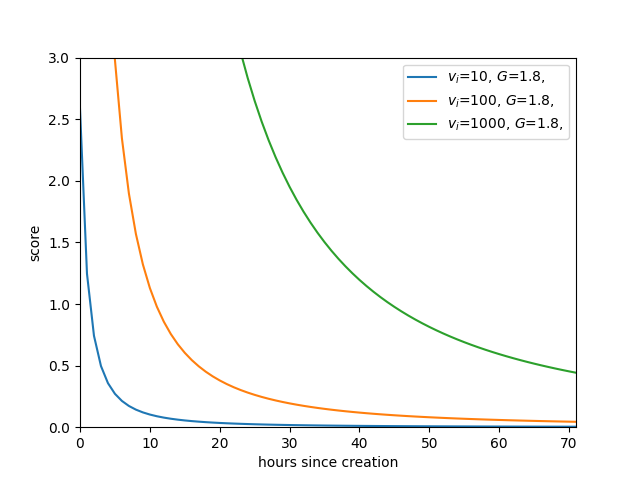
\includegraphics[width=\textwidth]{images/time_ranking_1.png}
    \caption{different views number}
  \end{subfigure}
  \hfill
  \begin{subfigure}[b]{0.5\textwidth}
    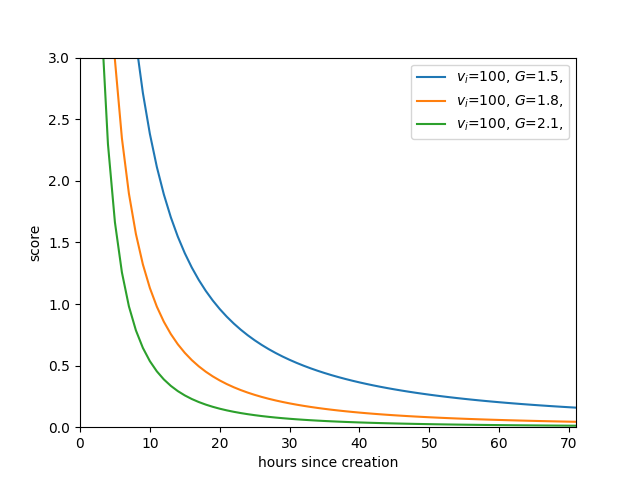
\includegraphics[width=\textwidth]{images/time_ranking_2.png}
    \caption{different gravity factor}
  \end{subfigure}
\caption{time-based ranking scoring}
    \label{fig:samples}
\end{figure}


At the end scores are normalized by \texttt{min-max} normalization.


\subsubsection{Content-based filtering (categories)}

As was told before, content-based filtering have its own impact weight, which is small at start (we don't want to restrict user from content just because he made some random clicks), but it inscreases as user interacts with the system and we may make predictions about his categorial preferences.

\subsection{Ranking components overview}



\subsubsection{Collaborative filtering}

We are using SVD++ algorithm.

For collaborative filtering recommendation we should have something known as user-item matrix which may be formed from user activity from tables (cite tables)

\subsubsection{Popularity filtering}

For measuring news item popularity following data can be aggregated: \hyperref[tab:show]{shows}, \hyperref[tab:view]{views}, \hyperref[tab:emotion]{emotions}, \hyperref[tab:comment]{comments}.

\begin{table}[h]
    \centering
    % \resizebox{\textwidth}{!}{
    \begin{tabular}{ccccc}
        \toprule

        \emph{item\_id} & \emph{shows\_num} & \emph{views\_num} & \emph{emotions\_num} & \emph{comments\_num} \\\midrule

        1 & 1043 & 231 & 52 & 7  \\
        2 & 828  & 478 & 78 & 11 \\
        3 & 163  & 25  & 5  & 0  \\
        \vdots & \vdots & \vdots & \vdots & \vdots \\\bottomrule


     \hline
    \end{tabular}
    % }

    \caption{aggregated popularity data}
    \label{tab:popularity}
\end{table}


\subsubsection{Session filtering}

\subsubsection{Content-based filtering}

\section{Implementation}
\label{sec:implementation}

\section{Evaluation}
\label{sec:evaluation}

    For evaluation we have information about what recommendation list was given to each user, and what is the source of the recommendation:

    \begin{table}[h]
        \centering
        \begin{tabular}{cccc}
            \toprule
            \textit{user\_id} & \textit{recommendation\_list}       & \textit{content\_based\_filtering}  & \textit{collaborative\_filtering} \\
            \midrule
            2 & \{(2, 0.91), (1, 0.74), (3, 0.23)\} & \{(2, 0.45), (1, 0.54), (3, 0.08)\} & \{(2, 0.92), (1, 0.4), (3, 0.3)\}\\

            1 & \{(3, 0.73), (1, 0.69), (2, 0.15)\} & \{(2, 0.6), (1, 0.44), (3, 0.04)\} & \{(2, 0.58), (1, 0.58), (3, 0.14)\}\\
            \vdots & \vdots & \vdots & \vdots \\
            \bottomrule
        \end{tabular}%
        
        \caption{recommendations' logs}
        \label{tab:recommendation_logs}
    \end{table}

    \begin{itemize}
        \item \textit{recommendation\_list}: list of recommendations that consists of pairs (\textit{item\_id}, \textit{score})
        \item \textit{content\_based\_filtering \& collaborative\_filtering}: sources of recommendation
    \end{itemize}

    As we use weighted sum of our recommmenders, we have unique boost values for every user:

    \begin{table}[h]
        \centering
        \begin{tabular}{ccc}
            \toprule
            \textit{user\_id} & \textit{content\_based\_filtering} & \textit{collaborative\_filtering} \\
            \midrule
            1                 & 0.25                                  & 1                               \\
            2                 & 1                               & 0.5                                \\
            \vdots & \vdots & \vdots \\
            \bottomrule
            \end{tabular}%
        \caption{boost values}
        \label{tab:boost_values}
    \end{table}

    To illustrate score calculation of recommendations, take a look at 1st row of table \hyperref[tab:recommendation_logs]{recommendations' logs}. We see recommendation $r = \{(2, 0.91), (1, 0.74), (3, 0.23)\}$ for user $u = 2$, so we should find boost values for this particular user in table \hyperref[tab:boost_values]{boost values}: content-based filtering boost $b_{cbf}$ for $u$ is $1$, collaborative filtering boost $b_{cf}$ is $0.5$. So final score is calculated in the following way: $0.91 = 0.45 * b_{cbf} + 0.92 * b_{cf} = 0.45 * 1 + 0.92 * 0.5 = 0.45 + 0.46$.

    Also we have information about \hyperref[tab:show]{shows} and \hyperref[tab:view]{views}, so we are able to track what item in recommendation list was clicked and what item was skipped, so depending on this information we can track if user liked item or not.



\subsection{Online}

\subsection{Offline}

\section{Further research}
\label{sec:further}

\section{Summary}
\label{sec:summary}

    Results show that combining different approaches leads to rise of users' involvement.

    

\bibliographystyle{unsrtnat}
\bibliography{references}  

\end{document}
